\documentclass[aps, preprint, prb,]{revtex4-2}
\usepackage{amsmath, amssymb, graphicx}
\usepackage{comment}
\graphicspath{{images}}
\usepackage{subcaption}
\usepackage{adjustbox}
\usepackage{float}
\usepackage{dcolumn} % Align table columns on the decimal point
\usepackage{bm} %Bold math 
\usepackage{booktabs} % For professional table formatting
\usepackage{makecell}
\usepackage{multirow} % For multi-row cells
\usepackage{braket} % For \ket and related commands
\usepackage{ragged2e} % For \justifying
\usepackage[version=4]{mhchem}
\usepackage{verbatim}
\usepackage{xcolor}

\def\qq{\mathbf{q}}
\def\kk{\mathbf{k}}
\def\KK{\mathbf{K}}
\def\DKK{\Delta\mathbf{K}}
\def\pp{\mathbf{p}}
\def\RR{\mathbf{R}}
\def\tt{\mathbf{t}}
\def\rr{\mathbf{r}}
\def\GG{\mathbf{G}}
\def\QQ{\mathbf{Q}}
\def\aa{\mathbf{a}}
\def\bb{\mathbf{b}}
\def\uu{\mathbf{u}}
\def\PP{\mathbf{P}}

\def\KK{\mathbf{K}}
\def\qq{\mathbf{q}}
\def\pp{\mathbf{p}}
\def\pp{\mathbf{p}}
\def\GG{\mathbf{G}}
\def\QQ{\mathbf{Q}}
\def\RR{\mathbf{R}}
\def\tt{\mathbf{t}}
\def\dd{\mathbf{d}}
\def\aa{\mathbf{a}}
\def\bb{\mathbf{b}}
\def\ee{\epsilon}
\def\CC{\mathcal{P}}
\def\gs{{\bs g}}

\def\BZ{{\rm BZ}}
\def\mS{{\mathcal{S}}}
\begin{document}

This Supporting Information provides additional computational details and screening results for the candidate heterostructures in other families.
\section{$P\bar{6}m2$ family}
For the symmetry group $P\bar{6}m2$ we choose HgCl$_2$/TiTe$_2$ as an example. We adopt the same sequence of calculations as in the $P\bar{3}m1$ example. Without SOC, the monolayers again realize a type-II alignment: HgCl$_2$ provides the conduction edge and TiTe$_2$ provides the valence edge. The relevant $\Gamma$-point irreps in the scalar calculation are $\mathbf{\Gamma}_1^+$ for the HgCl$_2$ CBM and $\mathbf{\Gamma}_3^-$ for the TiTe$_2$ VBM, yielding an atomic offset gap of approximately $0.01$~eV. Turning on SOC within r2SCAN \cite{furness2020accurate}, we obtain the spinor labels at the band edges: the HgCl$_2$ CBM is assigned to $\bar{\mathbf{\Gamma}}_7$, while the TiTe$_2$ VBM belongs to $\bar{\mathbf{\Gamma}}_9$.

We then build the HgCl$_2$/TiTe$_2$ bilayer and compute the SOC band structure for the reference (non-moir\'e) configuration. The absence of inversion in the stacked geometry reduces the point group from $D_{3h}$ in the monolayers to $C_{3v}$ in the heterostructure. The resulting r2SCAN+SOC band structure shows a direct gap of $0.11$~eV at $\Gamma$ with type-II alignment (Fig.~\ref{hgcl2_tite2}). The TiTe$_2$-dominated VBM transforms as $\bar{\mathbf{\Gamma}}_5 \bar{\mathbf{\Gamma}}_6$ with $J_z=\pm \frac{3}{2}$, whereas the HgCl$_2$-dominated CBM carries $\bar{\mathbf{\Gamma}}_4$ with $J_z=\pm \frac{1}{2}$.

\begin{figure}
 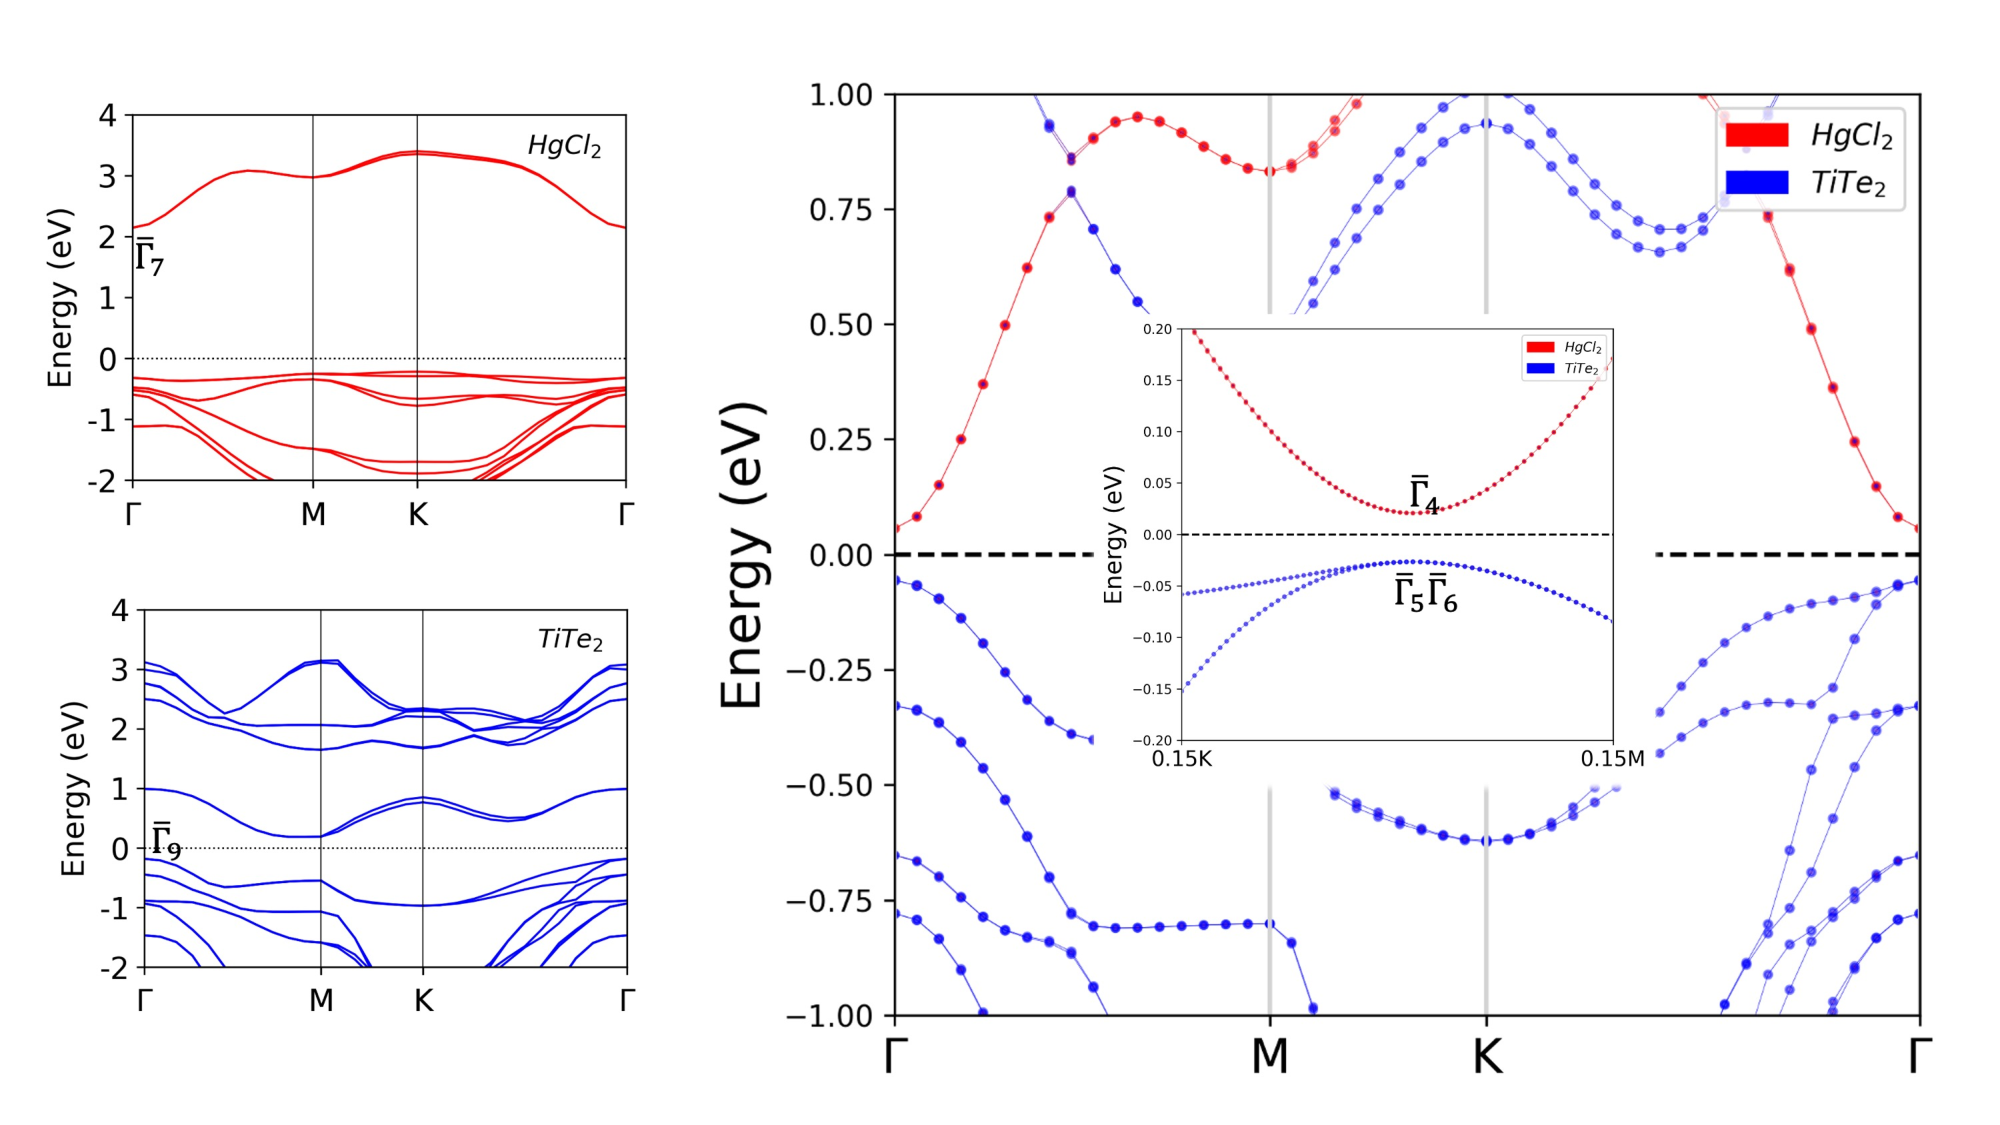
\includegraphics[width=1.0\textwidth]{images/hgcl2_tite2_bands_layer_resolved.pdf}
 \caption{Layer-resolved band structure of HgCl$_2$/TiTe$_2$ including SOC. The $\Gamma$-point gap remains type-II, with the VBM on TiTe$_2$ and the CBM on HgCl$_2$.}
 \label{hgcl2_tite2}
\end{figure}
\begin{table}[htbp]
\centering
\caption{Candidate material pairs for type-II heterostructures in $P\bar{6}m2$ including lattice constants, band edges (CBM/VBM) with irreducible representations (IRs), type-II energy gap, and lattice mismatch.}
\renewcommand{\arraystretch}{1.2}
\setlength{\tabcolsep}{4pt}
\resizebox{\textwidth}{!}{%
\begin{tabular}{c c c c c c c c}
\toprule
\textbf{Material 1} & Lattice const. (\AA) & CBM$_{M1}$ (eV) (IR) & \textbf{Material 2} & Lattice const. (\AA) & VBM$_{M2}$ (eV) (IR) & $\Delta E$ (eV) & Mismatch (\%) \\
\midrule
HgCl$_2$    & 3.803 & $-5.61$ ($\Gamma_1$)  & TiTe$_2$  & 3.737 & $-5.839$ ($\Gamma_5$) & 0.229 & $-1.74$ \\
PbO$_2$     & 3.265 & $-8.599$ ($\Gamma_1$) & ZnCl$_2$  & 3.480 & $-8.661$ ($\Gamma_5$) & 0.062 & $ 6.58$ \\
Tl$_2$S$_2$ & 4.057 & $-5.612$ ($\Gamma_4$) & TiTe$_2$  & 3.737 & $-5.839$ ($\Gamma_5$) & 0.227 & $-7.89$ \\
PbO$_2$     & 3.265 & $-8.599$ ($\Gamma_1$) & MgCl$_2$  & 3.557 & $-9.024$ ($\Gamma_5$) & 0.425 & $ 8.94$ \\
HgBr$_2$    & 3.976 & $-5.27$ ($\Gamma_1$)  & InN       & 3.575 & $-5.404$ ($\Gamma_6$) & 0.134 & $-10.09$ \\
Tl$_2$Se$_2$& 4.223 & $-5.373$ ($\Gamma_4$) & TiTe$_2$  & 3.737 & $-5.839$ ($\Gamma_5$) & 0.466 & $-11.51$ \\
Tl$_2$Se$_2$& 4.223 & $-5.373$ ($\Gamma_4$) & InN       & 3.575 & $-5.404$ ($\Gamma_6$) & 0.031 & $-15.34$ \\
Tl$_2$Se$_2$& 4.223 & $-5.373$ ($\Gamma_4$) & PbSe$_2$  & 4.877 & $-5.717$ ($\Gamma_5$) & 0.344 & $ 15.49$ \\
Tl$_2$S$_2$ & 4.057 & $-5.612$ ($\Gamma_4$) & PbS$_2$   & 4.727 & $-6.018$ ($\Gamma_5$) & 0.406 & $ 16.51$ \\
Tl$_2$S$_2$ & 4.057 & $-5.612$ ($\Gamma_4$) & PbSe$_2$  & 4.877 & $-5.717$ ($\Gamma_5$) & 0.105 & $ 20.21$ \\
Tl$_2$Te$_2$& 4.511 & $-4.907$ ($\Gamma_4$) & InN       & 3.575 & $-5.404$ ($\Gamma_6$) & 0.497 & $-20.75$ \\
HgBr$_2$    & 3.976 & $-5.27$ ($\Gamma_1$)  & PbSe$_2$  & 4.877 & $-5.717$ ($\Gamma_5$) & 0.447 & $ 22.66$ \\
HgCl$_2$    & 3.803 & $-5.61$ ($\Gamma_1$)  & PbS$_2$   & 4.727 & $-6.018$ ($\Gamma_6$) & 0.408 & $ 24.30$ \\
\bottomrule
\end{tabular}%
}
\label{tab:p-6m2}
\end{table}

\section{ $P\bar{4}m2$ family}
For the tetragonal $P\bar{4}m2$ group, we study the PbS$_2$/TiTe$_2$ heterostructure. We start from the monolayers and compute the r2SCAN band structures with SOC, then identify the band-edge irreps at $\Gamma$. The type-II alignment is already clear at the monolayer level: the CBM comes from PbS$_2$ and the VBM comes from TiTe$_2$. At $\Gamma$, the PbS$_2$ CBM has irrep $\mathbf{\Gamma}_6$, while the TiTe$_2$ VBM has irrep $\mathbf{\Gamma}_7$ (Fig.~\ref{pbs2_tite2}). The band-edge angular-momentum character is consistent with these assignments: the CBM is mainly $J_z=\pm \tfrac{1}{2}$ and the VBM is mainly $J_z=\pm \tfrac{3}{2}$.

Next, we build the PbS$_2$/TiTe$_2$ bilayer and compute the band structure with r2SCAN+SOC. In the monolayers the point group at $\Gamma$ is $D_{2d}$, but the heterostructure breaks inversion symmetry and reduces it to $C_{2v}$. The heterostructure keeps the same type-II ordering: the CBM remains on the PbS$_2$ layer and the VBM remains on the TiTe$_2$ layer, as seen from the layer-resolved bands (Fig.~\ref{pbs2_tite2}). At $\Gamma$, both band edges in the heterostructure are labeled by $\mathbf{\Gamma}_5$ in $C_{2v}$, while their dominant angular momentum character stays different: $J_z=\pm \tfrac{1}{2}$ for the CBM and $J_z=\pm \tfrac{3}{2}$ for the VBM. These symmetry labels and layer characters define the band-edge basis used in the low-energy model.

\begin{table}[htbp]
\centering
\caption{Candidate material pairs for type-II heterostructures in $P\bar{4}m2$ space group including their lattice constants, band edges (CBM/VBM) with irreducible representations (IRs), type-II energy gap, and lattice mismatch.}
\renewcommand{\arraystretch}{1.2}
\setlength{\tabcolsep}{4pt}
\resizebox{\textwidth}{!}{%
\begin{tabular}{c c c c c c c c}
\toprule
\textbf{Material 1} & Lattice const. (\AA) & CBM$_{M1}$ (eV) (IR) & \textbf{Material 2} & Lattice const. (\AA) & VBM$_{M2}$ (eV) (IR) & $\Delta E$ (eV) & Mismatch (\%) \\
\midrule
HgF$_2$  & 3.940 & $-5.682$ ($\Gamma_1$) & TiTe$_2$ & 4.123 & $-5.805$ ($\Gamma_5$) & 0.123 & 4.64 \\
PbS$_2$  & 3.933 & $-5.344$ ($\Gamma_1$) & TiTe$_2$ & 4.123 & $-5.805$ ($\Gamma_5$) & 0.461 & 4.83 \\
HgF$_2$  & 3.940 & $-5.682$ ($\Gamma_1$) & HfTe$_2$ & 4.282 & $-5.979$ ($\Gamma_5$) & 0.297 & 8.68 \\
HgF$_2$  & 3.940 & $-5.682$ ($\Gamma_1$) & ZrTe$_2$ & 4.307 & $-5.951$ ($\Gamma_5$) & 0.269 & 9.31 \\
PbO$_2$  & 3.537 & $-6.715$ ($\Gamma_1$) & HfSe$_2$ & 4.010 & $-6.774$ ($\Gamma_5$) & 0.059 & 13.37 \\
PbO$_2$  & 3.537 & $-6.715$ ($\Gamma_1$) & NiCl$_2$ & 4.091 & $-7.146$ ($\Gamma_5$) & 0.431 & 15.66 \\
\bottomrule
\end{tabular}%
}
\label{tab:p-4m2}
\end{table}
\section{$P3m1$}
The $P3m1$ candidates, shown in Table~\ref{tab:p3m1}, also have a trigonal setting with polar symmetry. Compared with the $P\bar{3}m1$ family, these systems show that the same design principle is applicable even when the global symmetry changes from centrosymmetric to polar.
\begin{table}[htbp]
\centering
\caption{Candidate material pairs for type-II heterostructures in $P3m1$ group including their lattice constants, band edges (CBM/VBM) with irreducible representations (IRs), type-II energy gap, and lattice mismatch.}
\renewcommand{\arraystretch}{1.2}
\setlength{\tabcolsep}{4pt}
\resizebox{\textwidth}{!}{%
\begin{tabular}{c c c c c c c c}
\toprule
\textbf{Material 1} & Lattice const. (\AA) & CBM$_{M1}$ (eV) (IR) & \textbf{Material 2} & Lattice const. (\AA) & VBM$_{M2}$ (eV) (IR) & $\Delta E$ (eV) & Mismatch (\%) \\
\midrule
HgTe & 4.732 & $-5.062$ ($\Gamma_1$) & InSb & 4.663 & $-5.444$ ($\Gamma_3$) & 0.382 & $-1.46$ \\
HgS & 4.287 & $-5.289$ ($\Gamma_1$) & InAs & 4.352 & $-5.780$ ($\Gamma_3$) & 0.491 &  $1.52$ \\
HgSe & 4.464 & $-5.630$ ($\Gamma_1$) & InAs & 4.352 & $-5.780$ ($\Gamma_3$) & 0.150 & $-2.51$ \\
HgSe & 4.464 & $-5.630$ ($\Gamma_1$) & PbTe & 4.324 & $-5.957$ ($\Gamma_3$) & 0.327 & $-3.14$ \\
HgSe & 4.464 & $-5.630$ ($\Gamma_1$) & HgS & 4.287 & $-6.122$ ($\Gamma_3$) & 0.492 & $-3.97$ \\
HgSe & 4.464 & $-5.630$ ($\Gamma_1$) & HgTe & 4.732 & $-5.800$ ($\Gamma_3$) & 0.170 & $6.00$ \\
HgSe & 4.464 & $-5.630$ ($\Gamma_1$) & SnTe & 4.173 & $-5.935$ ($\Gamma_3$) & 0.305 & $-6.52$ \\
HgS & 4.287 & $-5.289$ ($\Gamma_1$) & GeTe & 3.943 & $-5.749$ ($\Gamma_3$) & 0.460 & $-8.02$ \\
PbO & 3.593 & $-4.964$ ($\Gamma_1$) & ZrSeTe & 3.884 & $-5.080$ ($\Gamma_3$) & 0.116 & $8.10$ \\
HgS & 4.287 & $-5.289$ ($\Gamma_1$) & InSb & 4.663 & $-5.444$ ($\Gamma_3$) & 0.155 & $8.77$ \\
HgSe & 4.464 & $-5.630$ ($\Gamma_1$) & AsITe & 3.961 & $-6.077$ ($\Gamma_3$) & 0.447 & $-11.27$ \\
HgSe & 4.464 & $-5.630$ ($\Gamma_1$) & GeTe & 3.943 & $-5.749$ ($\Gamma_3$) & 0.119 & $-11.67$ \\
HgS & 4.287 & $-5.289$ ($\Gamma_1$) & HfSTe & 3.716 & $-5.767$ ($\Gamma_3$) & 0.478 & $-13.32$ \\
HgSe & 4.464 & $-5.630$ ($\Gamma_1$) & AsISe & 3.826 & $-5.992$ ($\Gamma_3$) & 0.362 & $-14.29$ \\
HgSe & 4.464 & $-5.630$ ($\Gamma_1$) & ZrSeTe & 3.810 & $-6.115$ ($\Gamma_3$) & 0.485 & $-14.65$ \\
HgSe & 4.464 & $-5.630$ ($\Gamma_1$) & AsIS & 3.746 & $-5.933$ ($\Gamma_3$) & 0.303 & $-16.08$ \\
HgSe & 4.464 & $-5.630$ ($\Gamma_1$) & HfSTe & 3.716 & $-5.767$ ($\Gamma_3$) & 0.137 & $-16.76$ \\
HgTe & 4.732 & $-5.062$ ($\Gamma_1$) & ZrSeTe & 3.884 & $-5.080$ ($\Gamma_3$) & 0.018 & $-17.92$ \\
HgS & 4.287 & $-5.289$ ($\Gamma_1$) & TiSSe & 3.478 & $-5.509$ ($\Gamma_3$) & 0.220 & $-18.87$ \\
HgSe & 4.464 & $-5.630$ ($\Gamma_1$) & TiSTe & 3.546 & $-5.808$ ($\Gamma_3$) & 0.178 & $-20.56$ \\
\bottomrule
\end{tabular}%
}
\label{tab:p3m1}
\end{table}

\begin{figure}
 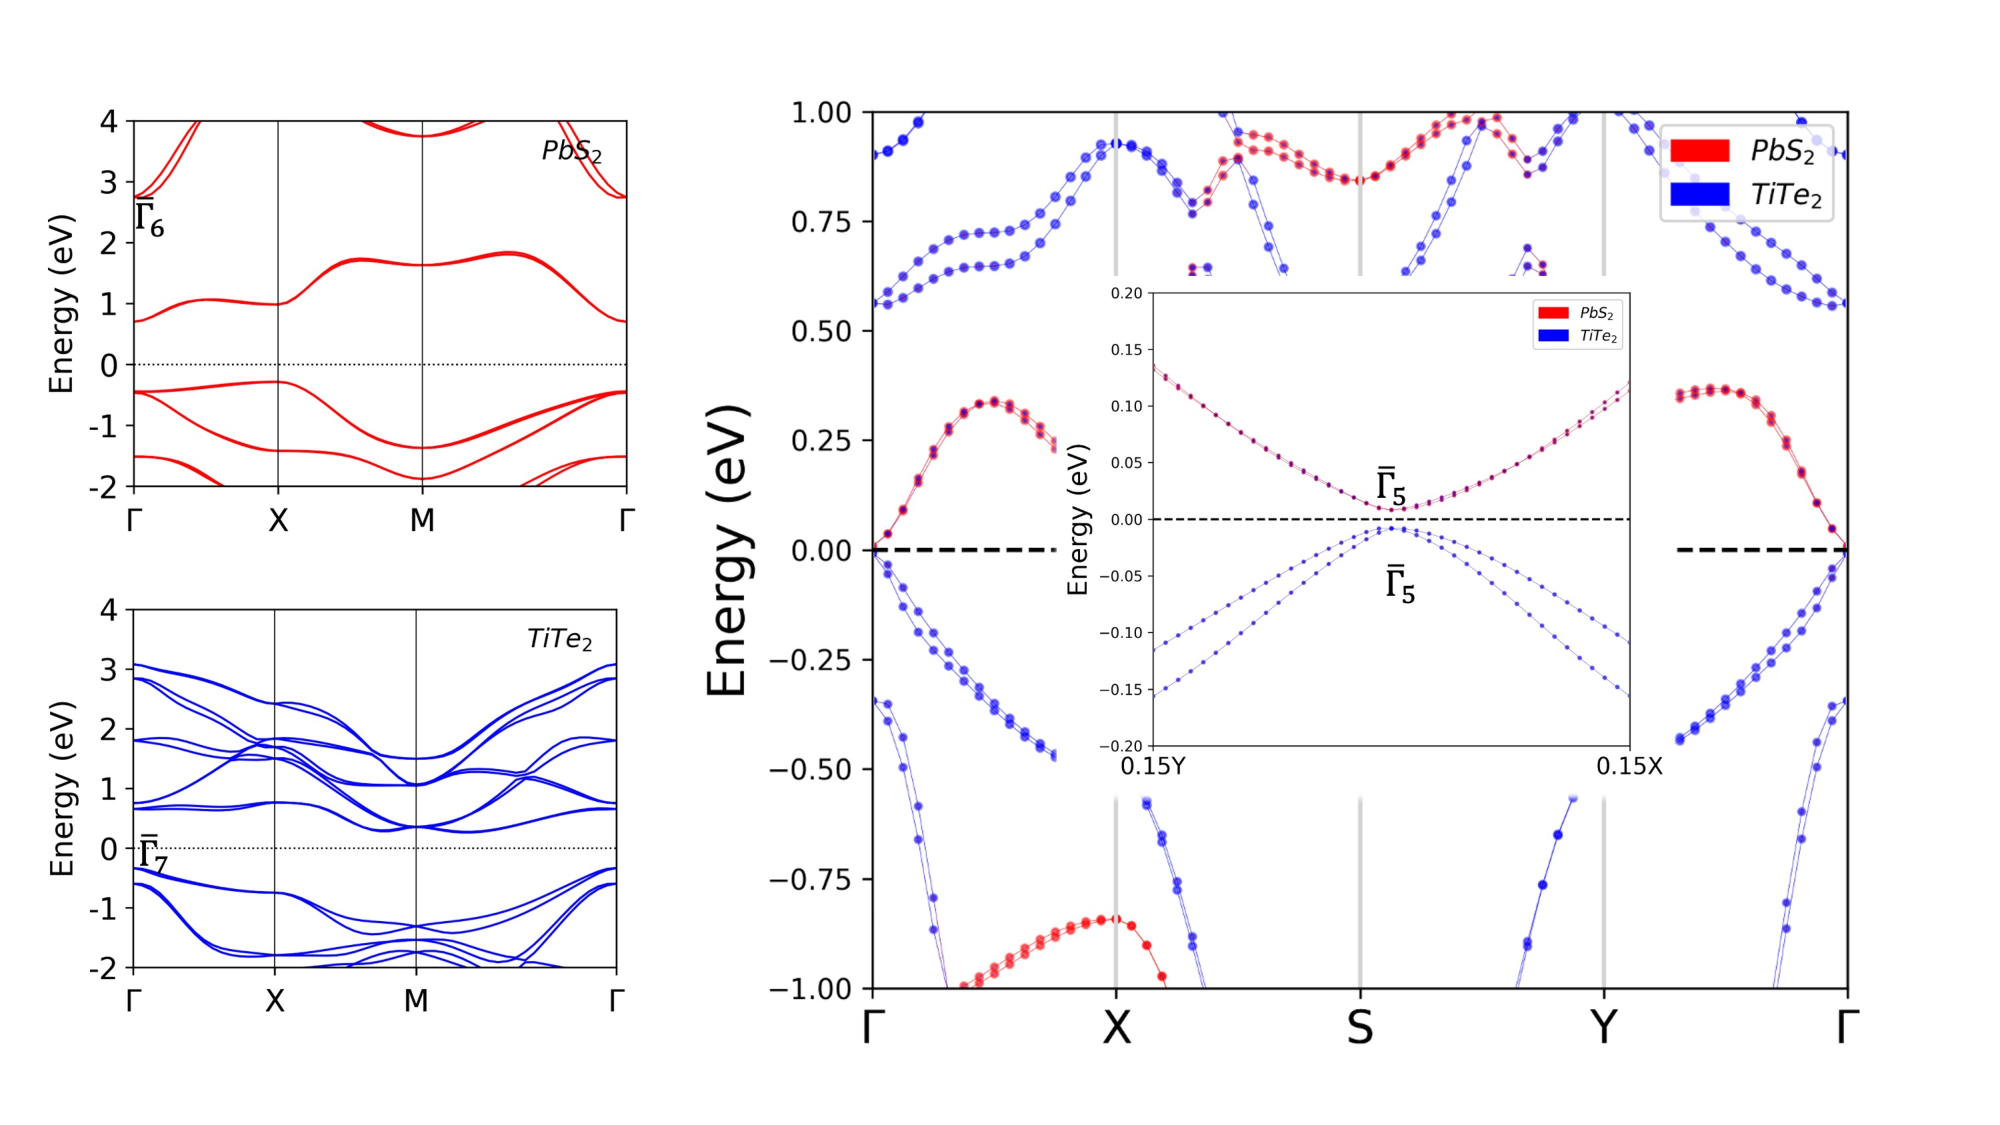
\includegraphics[width=1.0\textwidth]{images/pbs2_tite2_bands_layer_resolved.pdf}
 \caption{Layer-resolved band structure of PbS$_2$/TiTe$_2$ including SOC. The $\Gamma$-point gap remains type-II, with the VBM on TiTe$_2$ and the CBM on HgCl$_2$.}
 \label{pbs2_tite2}
\end{figure}

\section{NequIP-based relaxation and moir\'e-potential validation}
The continuum THF model introduced in the previous section establishes the conditions under which moir\'e minibands can host topological heavy-fermion physics.  A quantitative evaluation of the moir\'e potential is required to validate the candidate heterostructures identified from symmetry and band-alignment considerations. Realistic moir\'e supercells, particularly at small twist angles or for nearly lattice-matched systems, can contain thousands of atoms. Direct structural relaxation and potential evaluation using density functional theory (DFT) at this scale is computationally prohibitive. To overcome this limitation, we employ a machine-learned interatomic potential based on the NequIP framework \cite{Batzner2022NequIP}, which enables efficient and accurate exploration of the moir\'e structural landscape.

NequIP is an $E(3)$-equivariant graph neural network that maps local atomic environments to total energies and forces while preserving rotational and geometric symmetries. This property is particularly important for layered heterostructures, where interlayer registry, local coordination, and out-of-plane relaxation collectively determine the spatial variation of the moir\'e potential. The model is trained on a DFT-generated dataset consisting of representative bilayer configurations that sample interlayer translations, interlayer distances, and local distortions around aligned and near-aligned geometries.

For each configuration, DFT provides the total energy $E^{\mathrm{DFT}}$ and atomic forces $\mathbf{F}^{\mathrm{DFT}}$. The NequIP model predicts $E^{\mathrm{pred}}$ and $\mathbf{F}^{\mathrm{pred}}$ by constructing symmetry-equivariant features from the atomic neighborhood. The training objective is defined as a combined energy-force loss,
\begin{equation}
\mathcal{L} =
w_E \left| E^{\mathrm{pred}} - E^{\mathrm{DFT}} \right|^2
+
w_F \frac{1}{N}\sum_{i=1}^{N}
\left\| \mathbf{F}_i^{\mathrm{pred}} - \mathbf{F}_i^{\mathrm{DFT}} \right\|^2,
\end{equation}
where $N$ is the number of atoms in the configuration.

Once trained, the NequIP potential is used to relax large moir\'e supercells corresponding to selected candidate heterostructures. These relaxed structures capture the spatial variation of interlayer distance and local stacking registry across the moir\'e unit cell, which are the primary structural factors governing the moir\'e modulation.

To obtain the electronic moir\'e potential, we return to first-principles calculations. Density functional theory (DFT) calculations are performed within VASP \cite{Kresse1996VASP} on representative relaxed configurations extracted from the moir\'e supercell. The electrostatic potential is then evaluated in regions located at a distance $d$ away from the outermost atomic layers of the bilayer. Specifically, we define reference planes using the average $z$-coordinates of the topmost and bottommost atoms, denoted by $z_{\mathrm{top}}$ and $z_{\mathrm{bot}}$, respectively. The potentials are sampled at
\begin{equation}
z = z_{\mathrm{top}} + d, \quad \text{and} \quad z = z_{\mathrm{bot}} - d,
\end{equation}
ensuring that the evaluation region lies outside the atomic cores while remaining sensitive to the local electronic environment.

The resulting planar-resolved potentials,
\begin{equation}
V_{\mathrm{top}}(\mathbf{r}), \quad V_{\mathrm{bot}}(\mathbf{r}),
\end{equation}
provide a spatial map of the moir\'e modulation across the supercell. From the perspective of the THF model, the critical quantity is the layer-dependent variation of this potential. A viable THF system requires a strongly asymmetric modulation, in which one sector (typically the valence-derived band) experiences significant localization while the other remains relatively dispersive.

By analyzing the amplitude and spatial variation of these layer-resolved potentials across high-symmetry stacking regions, we assess whether the effective moir\'e potential assumed in the continuum model can be realized in the candidate heterostructures. In this way, the combination of NequIP-based structural relaxation and DFT-based potential extraction provides a quantitative validation of the theoretical design principle, linking atomic-scale energetics to emergent moir\'e-scale physics.
In the present validation study, we use twisted bilayer \ce{PtTe2} as a representative system for estimating the moir\'e electrostatic potential. We first construct \(2\times2\) bilayer supercells of \ce{PtTe2} and generate a set of laterally shifted bilayer configurations to sample different local stacking registries. Each shifted structure is relaxed using VASP with the r2SCAN exchange-correlation functional and van der Waals corrections, so that both the intralayer bonding and interlayer relaxation are treated consistently. From 400 shifted bilayer structures, we generate a training dataset containing 30,697 atomic configurations with corresponding energies and forces. This dataset is used to train the NequIP interatomic potential with a cutoff radius of \(4.0~\text{\AA}\), five equivariant interaction layers, \(l_{\max}=3\), and 64 features. The trained model is then used to relax larger twisted \ce{PtTe2} moir\'e supercells efficiently before performing self-consistent VASP calculations to extract the spatial variation of the electrostatic potential.
\section{Effective model}
\subsection{$P\bar{3}m1$}
In space group $P\bar{3}m1$, the little group at $\Gamma$ is $D_{3d}$. When a heterostructure is formed, the little group is reduced to $C_{3v}$. The character tables for  these two groups are shown in Tab.~\ref{Tab:charter table D3d c3v}(a) and (c). When the SOC is not included, according to the compatibility relation, the $\mathbf{\Gamma}^+_1$ and $\mathbf{\Gamma}^-_3$ irreps of the $D_{3d}$ group for the conduction of HgCl$_2$ and the valence band of PtTe$_2$ correspond to the $\mathbf{\Gamma}_1$ and $\mathbf{\Gamma}_3$ irreps in the $C_{3v}$ group. When the SOC is included,  the irreps of conduction and valence bands are $\bar{\Gamma}_4$ and $\bar{\Gamma}_5\bar{\Gamma}_6$, respectively. Meanwhile, just as in the Tl$_2$Se$_2$/Zn$_2$Te$_2$ heterostructure, the conduction bands exhibit Rashba SOC.  Therefore, this case is exactly the same as the Tl$_2$Se$_2$/Zn$_2$Te$_2$ heterostructure in Ref.\cite{Liu2025IdealTHF}, and the effective model is given by
\begin{eqnarray}
&&H_{\mathrm{hetero}}(\kk)=
\begin{pmatrix}
H^{\uparrow\uparrow}_{\mathrm{hetero}}(\kk) & H^{\uparrow\downarrow}_{\mathrm{hetero}}(\kk) \\
\bigl(H^{\uparrow\downarrow}_{\mathrm{hetero}}(\kk)\bigr)^\dagger & H^{\downarrow\downarrow}_{\mathrm{hetero}}(\kk)
\end{pmatrix},\nonumber\\
&&H^{\uparrow\uparrow}_{\mathrm{hetero}}(\kk)=
\begin{pmatrix}
E_1 + A_1 k^2 & i B_0 (k_x + i k_y) \nonumber \\
- i B_0 (k_x - i k_y) & E_2 + A_2 k^2
\end{pmatrix}, H^{\downarrow\downarrow}_{\mathrm{hetero}}(\kk)=
\bigl(H^{\uparrow\uparrow}_{\mathrm{hetero}}(-\kk)\bigr)^*, \\
&&H^{\uparrow\downarrow}_{\mathrm{hetero}}(\kk)=
\begin{pmatrix}
- i R_0 k_- & 0 \\
0 & 0
\end{pmatrix}. \label{Eq;Rashba}
\end{eqnarray}

 By choosing the parameters $E_1=-E_2=0.045$~eV, $A_1=0.289~a_0^2\!\cdot\!\mathrm{eV}$, $B_0=0.257~a_0\!\cdot\!\mathrm{eV}$, $A_2=-0.434~a_0^2\!\cdot\!\mathrm{eV}$, and $R_0=0.134~a_0\!\cdot\!\mathrm{eV}$, we obtain the band dispersions from the effective model, shown as the orange curves in Fig.~\ref{fig:fit_p-3m1}. The effective model captures the low-energy band dispersions of the heterostructure well. 


\begin{figure}[htbp]
 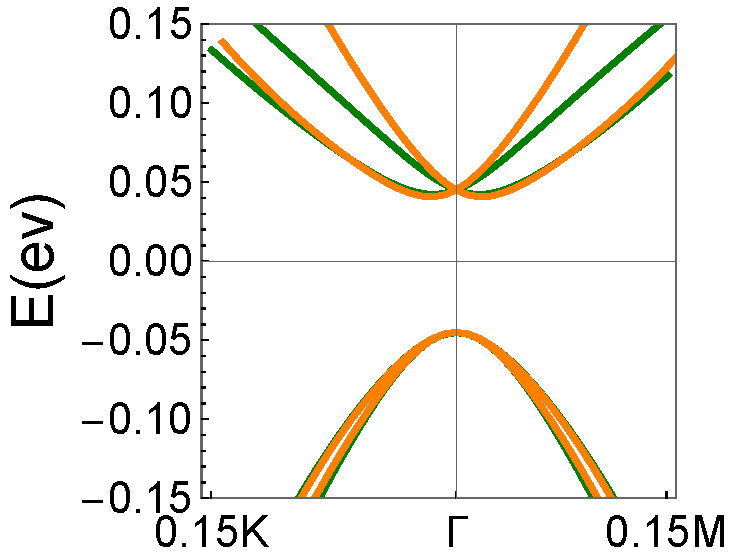
\includegraphics[width=0.5\textwidth]{images/fit_p-3m1.pdf}
 \caption{\justifying  A zoomed-in view of the band dispersion near $\mathbf{\Gamma}$ point from DFT calculation (green curves) and the corresponding effective model fitting (orange curves).}
 \label{fig:fit_p-3m1}
\end{figure}

\begin{table}[h]






\centering
\begin{subtable}{1\textwidth}
\centering
\renewcommand{\arraystretch}{1.2}
\begin{tabular}{|c|c|c|c|c|c|c|c|c|c|c|c|c|}
\hline
$D_{3d}$ & $\mathbf{\Gamma}_1^+$ & $\mathbf{\Gamma}_2^+$ & $\mathbf{\Gamma}_3^+$ & $\mathbf{\Gamma}_1^-$ & $\mathbf{\Gamma}_2^-$ & $\mathbf{\Gamma}_3^-$ & $\bar{\mathbf{\Gamma}}_4^+$ & $\bar{\mathbf{\Gamma}}_5^+$ & $\bar{\mathbf{\Gamma}}_6^+$ & $\bar{\mathbf{\Gamma}}_4^-$ & $\bar{\mathbf{\Gamma}}_5^-$ & $\bar{\mathbf{\Gamma}}_6^-$ \\
\hline
$E$& 1 & 1 & 2 & 1 & 1 & 2 & 2 & 1 & 1 & 2 & 1 & 1 \\
$2C_3$      & 1 & 1 & -1 & 1 & 1 & -1 & 1 & -1 & -1 & 1 & -1 & -1 \\
$3C_2$& 1 & -1 & 0 & 1 & -1 & 0 & 0 & $i$ & $-i$ & 0 & $i$ & $-i$ \\
$I$ & 1 & 1 & 2 & -1 & -1 & -2 & 2 & 1 & 1 & -2 & -1 & -1 \\
$2IC_3$& 1 & 1 & -1 & -1 & -1 & 1 & 1 & -1 & -1 & -1 & 1 & 1 \\
$3M_y$& 1 & -1 & 0 & -1 & 1 & 0 & 0 & $i$ & $-i$ & 0 & $-i$ & $i$ \\
\hline
\end{tabular}
\caption{\centering }
\end{subtable} 


\begin{subtable}{1\textwidth}
\centering
\renewcommand{\arraystretch}{1.2}
\begin{tabular}{|c|c|c|c|c|c|c|c|c|c|}
\hline
$D_{3h}$ & $\Gamma_1$ & $\Gamma_2$ & $\Gamma_3$ & $\Gamma_4$ & $\Gamma_5$ & $\Gamma_6$ & $\Bar{\Gamma}_7$ & $\Bar{\Gamma}_8$ & $\bar{\Gamma}_9$ \\
\hline
$E$        & 1 & 1 & 1  & 1  & 2  & 2  & 2  & 2 & 2 \\
$2C_3$     & 1 & 1 & 1  & 1  & -1 & -1 & -2 & 1 & 1 \\
$M_z$      & 1 & 1 & -1 & -1 & 2  & -2 & 0  & 0 & 0 \\
$2IC_6$    & 1 & 1 & -1 & -1 & -1 & 1  & 0  & -$\sqrt{3}$ & $\sqrt{3}$ \\
$3M_y$    & 1 & -1 & 1  & -1 & 0  & 0  & 0  & 0 & 0 \\
$3C_2$    & 1 & -1 & -1 & 1  & 0  & 0  & 0  & 0 & 0 \\
\hline
\end{tabular}
\caption{\centering }
\end{subtable} 

\begin{subtable}{1\textwidth}
\centering

\renewcommand{\arraystretch}{1.2}
\begin{tabular}{|c|c|c|c|c|c|c|}
\hline
$C_{3v}$ & $\mathbf{\Gamma}_1$ & $\mathbf{\Gamma}_2$ & $\mathbf{\Gamma}_3$ & $\bar{\mathbf{\Gamma}}_4$ & $\bar{\mathbf{\Gamma}}_5$ & $\bar{\mathbf{\Gamma}}_6$ \\
\hline
$E$ & 1 & 1 & 2 & 2 & 1 & 1 \\
$2C_3$ & 1 & 1 & $-1$ & 1 & $-1$ & $-1$ \\
$3IM_y$ & 1 & $-1$ & 0 & 0 & $i$ & $-i$ \\
\hline
\end{tabular}

\caption{\centering   }


\end{subtable}
\hfill
\caption { \justifying Character tables for the point groups $D_{3d}$, $D_{3h}$ and $C_{3v}$ in (a), (b) and (c), respectively. The irreps with a bar denote double (spinful) representations, while those without a bar correspond to single (spinless) representations.}
\label{Tab:charter table D3d c3v}
\end{table}
\subsection{$P\bar{6}m2$} \label{Sec: P6m2}
In space group $P\bar{6}m2$, the little group at $\Gamma$ is $D_{3h}$. When a heterostructure is formed, the little group is reduced to $C_{3v}$. The character table for $D_{3h}$ is shown in Tab.~\ref{Tab:charter table D3d c3v}(b). In this group, we consider the HgCl$_2$/TiTe$_2$ heterostructure. Without SOC, according to the compatibility relations, the $\mathbf{\Gamma}_1$ and $\mathbf{\Gamma}_5$ irreps of the $D_{3h}$ group for the conduction band of HgCl$_2$ and the valence band of TiTe$_2$ correspond to the $\mathbf{\Gamma}_1$ and $\mathbf{\Gamma}_3$ irreps of the $C_{3v}$ group, respectively. When SOC is included, the irreps of the conduction and valence bands become $\bar{\Gamma}_4$ and $\bar{\Gamma}_5\bar{\Gamma}_6$, respectively. In contrast to heterostructures whose parent materials belong to the $P\bar{3}m1$ group, the SOC splitting in the valence bands appears along the $\Gamma \text{K}$ direction rather than the $\Gamma \text{M}$ direction, as shown in Fig.~\ref{fig:P-6m2fit}(b). This indicates the presence of trigonal-warping SOC. We note that this type of SOC splitting already exists in TiTe$_2$. Therefore, we believe this SOC splitting originates from the TiTe$_2$ layer. Therefore, we are going to derive the effective mode for the valence bands of TiTe$_2$.

For the TiTe$_2$ layer, the band irrep of valence bands at $\Gamma$ is $\Bar{\Gamma}_9$. The representation matrix of the generators of group $D_{3h}$ is given by

\begin{eqnarray}
D(C_{3z})=
\begin{pmatrix}
-1 & 0\\
0 & -1
\end{pmatrix},\qquad
D(M_y)=
\begin{pmatrix}
0 & -1\\
1 & 0
\end{pmatrix},\qquad
D(M_z)=
\begin{pmatrix}
-i & 0\\
0 & i
\end{pmatrix}.
\end{eqnarray}
The $M_y$ operation changes $k_y$ to $-k_y$, and the $\Gamma\mathrm{M}$ direction lies in the mirror plane.

The two bands effective model takes the general form as
\begin{eqnarray}
    H_{V}(\kk)=\sum^{3}_{i=0}F^{ij}(\kk)\sigma_i,
\end{eqnarray}
 The $\sigma$ and $\lambda$ matrices transform as
\begin{eqnarray}
  &&D(C_{3z}) \sigma_i D^{-1}(C_{3z})=\sum_j\mathcal{D}^{ji}(C_{3z}) \sigma_j; 
  \\
  && D(M_{y}) \sigma_i D^{-1}(M_{y})=\sum_j\mathcal{D}^{ji}(M_{y}) \sigma_j;
  \\
   &&D(M_{z}) \sigma_i D^{-1}(M_{z})=\sum_j\mathcal{D}^{ji}(M_{z}) \sigma_j.
\end{eqnarray}


Using these representation matrices of $C_{3z}$, $M_y$, and $M_z$, we can compute the transformation matrices $\mathcal{D}$, from which we can classify the $\sigma$ and matrices into the irrep table of the $D_{3d}$ group, as shown in Table \ref{TAB: symmetry D3d matrix}.  Based on this table, we can write down the effective model as 
\begin{eqnarray} \label{eq:effective model D3d}
     H_{V}(\kk)=(a+bk^2)\sigma_0+w_3 k_y(k_x^2-3k_y^2) \sigma_3.
\end{eqnarray}
From Eq.~\ref{eq:effective model D3d}, we see that the only symmetry-allowed term up to $\kk^3$ order is the trigonal-warping SOC term. Taking the parameters $a=-0.14$~eV, $b=-0.266~a_0^2 \cdot \mathrm{eV}$, and $w_3=-0.164~a_0^3 \cdot \mathrm{eV}$, we obtain the band dispersions from the effective model for the TiTe$_2$ layer, shown as the orange curves in the inset of Fig.~\ref{fig:P-6m2fit}(a). The effective model captures the low-energy band dispersions of the TiTe$_2$ layer well.

Now we are going to write down the effective model for the heterostructure. By including the trigonal-warping SOC term, the effective model is given by
\begin{eqnarray}
&&H'_{\mathrm{hetero}}(\kk)=
\begin{pmatrix}
H'^{\uparrow\uparrow}_{\mathrm{hetero}}(\kk) & 0 \\
0 & H'^{\downarrow\downarrow}_{\mathrm{hetero}}(\kk)
\end{pmatrix},\nonumber\\
&&H'^{\uparrow\uparrow}_{\mathrm{hetero}}(\kk)=H^{\uparrow\uparrow}_{\mathrm{hetero}}(\kk)+
\begin{pmatrix}
0 & 0 \nonumber \\
0 &w_3 k_y(k_x^2-3k_y^2)
\end{pmatrix}, H’^{\downarrow\downarrow}_{\mathrm{hetero}}(\kk)=
\bigl(H‘^{\uparrow\uparrow}_{\mathrm{hetero}}(-\kk)\bigr)^*. \\
 \label{Eq;trigonal-warping}
\end{eqnarray}
Here $H^{\uparrow\uparrow}_{\mathrm{hetero}}(\kk)$ takes the same form as in Eq.~\ref{Eq;Rashba}. By choosing the parameters $E_1=-E_2=0.024$~eV, $A_1=0.467~a_0^2\!\cdot\!\mathrm{eV}$, $B_0=0.092~a_0\!\cdot\!\mathrm{eV}$, $A_2=-0.166~a_0^2\!\cdot\!\mathrm{eV}$, and $w_3=0.204~a_0^3\!\cdot\!\mathrm{eV}$, we obtain the band dispersions from the effective model, shown as the orange curves in Fig.~\ref{fig:P-6m2fit}(b). The effective model captures the low-energy band dispersions of the heterostructure well. The Hamiltonian $H'_{\mathrm{hetero}}(\kk)$ is spin-block-diagonal. If we ignore the cubic-order trigonal-warping term, $H'^{\uparrow\uparrow}_{\mathrm{hetero}}(\kk)$ can be transformed into $\hat{H}_{\rm BHZ}(\mathbf{k})$ in Eq.~2 in the main text by a unitary transformation.

\begin{table}[htbp]
\centering
\renewcommand{\arraystretch}{1.5}
\begin{tabular}{|c|c|c|c|}
\hline
\(D_{3d}\) & \(\sigma\) & \(k\) \\ 
\hline
\(\mathbf{\Gamma}_1 (A'_1)\)  & \(\sigma_0(+)\) & \(k_x^2 + k_y^2(+), \text{C}(+),k_x(k_x^2-3k_y^2)(-)\) \\
\hline 
\(\mathbf{\Gamma}_2 (A'_2)\)&  \(\sigma_3(-)\) & \( k_y(k_x^2-3k_y^2)(-)\)\\
\hline
\(\mathbf{\Gamma}_3 (A''_2)\)  & \(\sigma_1(-)\) &higher order  \\ 
\hline
\(\mathbf{\Gamma}_4 (A''_1)\)  &  \(\sigma_2(-)\) & higher order  \\
\hline 
\(\mathbf{\Gamma}_5 (E')\)&  & $(k_x,k_y)$ \\
\hline
\(\mathbf{\Gamma}_6 (E'')\)  &  & \((k_x,-k_y)(-)\), $(k^2_x-k^2_y, 2k_x k_y)(+)$ \\ 
\hline
\end{tabular}
\caption{\justifying  The classification of the representation matrices and $k$-polynomials for the $D_{3d}$ group. The + or - in the bracket indicates how the matrices transform under TR (even or odd). The symbol $\text{C}$ in the column of $k$-polynomial is for a constant. \label{TAB: symmetry D3d matrix} }
\end{table}

\begin{figure}[htbp]
 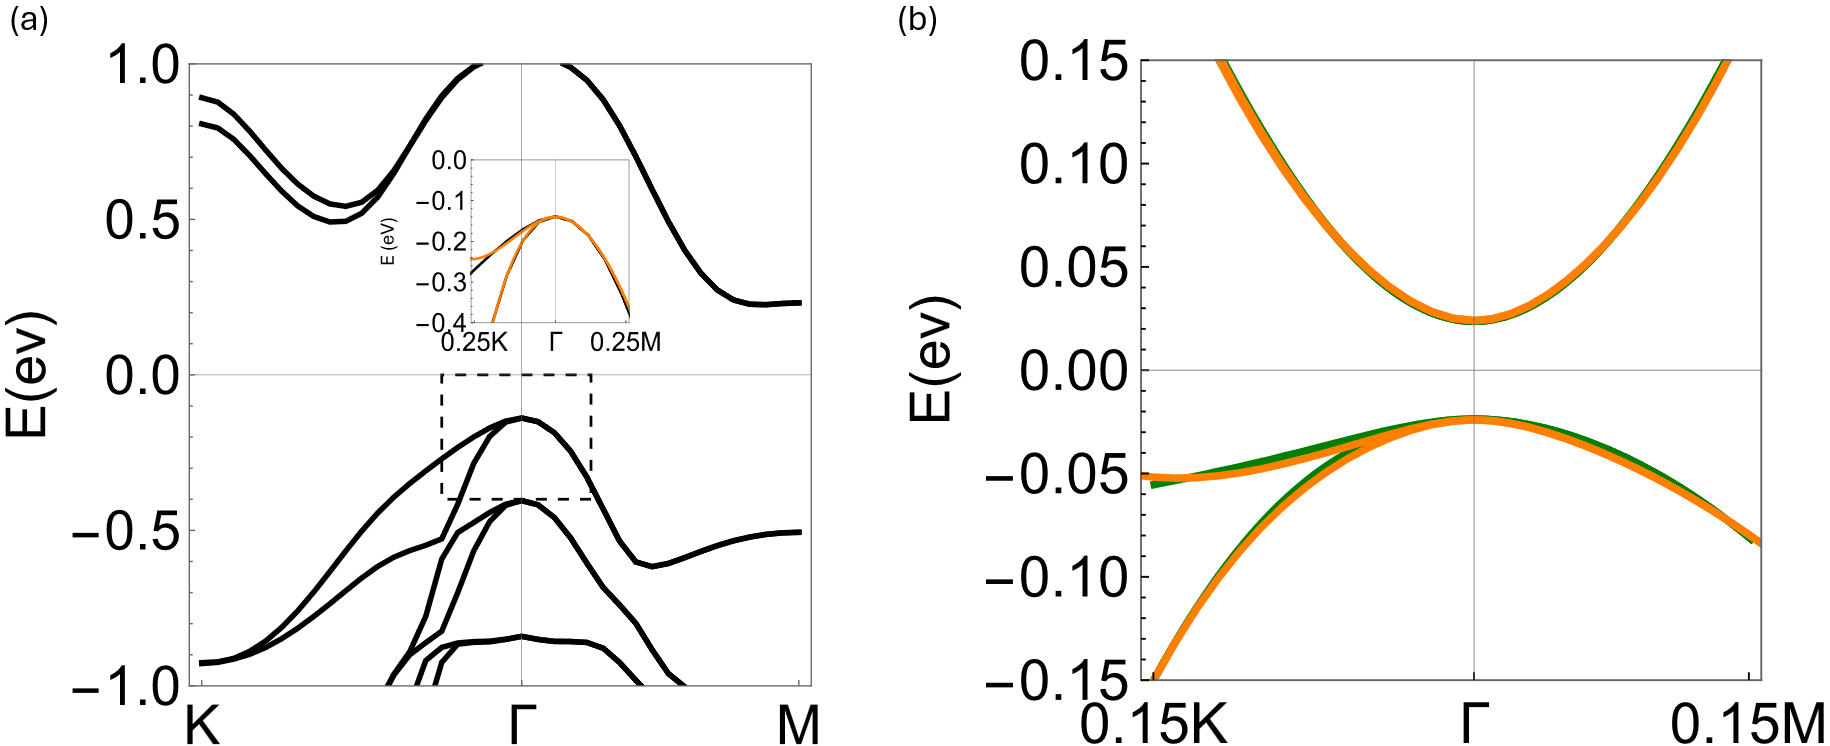
\includegraphics[width=1\textwidth]{images/P-6m2fit.png}
 \caption{\justifying (a) Band dispersion of TiTe$_2$. The inset shows a zoomed-in view of the band dispersion within the dashed box. The orange curves are obtained from the effective model. (b) A zoomed-in view of the band dispersion of the HgCl$_2$/TiTe$_2$ heterostructure near the $\mathbf{\Gamma}$ point from DFT calculations (green curves) and the corresponding effective-model fitting (orange curves).}
 \label{fig:P-6m2fit}
\end{figure}
\subsection{$P\bar{4}m2$}

In this section, we derive the effective model for the heterostructure whose parent materials belong to space group $P\bar{4}m2$.   The little group at $\Gamma$ is $D_{2d}$. When a heterostructure is formed, the little group is reduced to $C_{2v}$.  In this section, we consider the PbS$_2$/TiTe$_2$ heterostructure. Because the symmetry constraints in the $C_{2v}$ group are weaker, we adopt a different strategy to construct the effective model.  We first construct two band effective models based on the symmetry group $D_{2d}$ for the conduction bands of PbS$_2$ and the valence bands of TiTe$_2$. We then constrain the interlayer tunneling terms based on group $C_{2v}$. With SOC, the irreps of the conduction bands of PbS$_2$ and the valence bands of TiTe$_2$ are $\Bar{\Gamma}_6$ and $\Bar{\Gamma}_7$, respectively. 

The generators of group $D_{22}$ are $S_{4z}$ and $M_x$. According to the character table in Tab.~\ref{Tab:charter table D2d c2v}(a), the representation matrices of the generators  of $\bar{\Gamma}_7$ and $\bar{\Gamma}_6$ are 
\begin{eqnarray}
&&D_{\bar{\Gamma}_7}(S_{4z})=
\begin{pmatrix}
e^{-i3\pi/4} & 0\\
0 & e^{i3\pi/4}
\end{pmatrix},  
D_{\bar{\Gamma}_7}(M_x)=
\begin{pmatrix}
0 & 1\\
-1 & 0
\end{pmatrix},\\
&&D_{\bar{\Gamma}_6}(S_{4z})=
\begin{pmatrix}
e^{-i\pi/4} & 0\\
0 & e^{i\pi/4}
\end{pmatrix},  
D_{\bar{\Gamma}_6}(M_x)=
\begin{pmatrix}
0 & 1\\
-1 & 0
\end{pmatrix}.
\end{eqnarray}

We use the same method as that in Sec.~\ref{Sec: P6m2} to construct the effective Hamiltonians. Up to the second order, the two effective Hamiltonians take the same form, given by 
\begin{eqnarray}
H_{\mathrm{TiTe}_2(\mathrm{PbS}_2)}(\mathbf{k})=
\begin{pmatrix}
E_0+A(k_x^2+k_y^2) & R_0(k_x-i k_y)\\
R_0(k_x+i k_y) & E_0+A(k_x^2+k_y^2)
\end{pmatrix}.    
\end{eqnarray}

The off-diagonal term corresponds to the Rashba SOC term. For PbS$_2$, the Rashba SOC is negligible, as shown in Fig.~\ref{fig:P-4m2fit}(a). By choosing $E_0=-3.38$ eV and $A=0.534\,a_0^2\cdot\mathrm{eV}$, the effective model captures the low-energy conduction bands near $\Gamma$, as shown in Fig.~\ref{fig:P-4m2fit}(a). For TiTe$_2$, in contrast, the DFT band structure exhibits a significant Rashba splitting. By choosing appropriate fitting parameters $E_0=-3.054$ eV, $A=-0.566\,a_0^2\cdot\mathrm{eV}$ and $R_0=0.056\,a_0\cdot\mathrm{eV}$, the effective model captures the low-energy valence bands near $\Gamma$, as shown in Fig.~\ref{fig:P-4m2fit}(b).



Combining the two layers, the symmetry group is reduced to $C_{2v}$, and the irreps for both conduction bands and valence bands at $\Gamma$ are $\Bar{\Gamma}_5$. The heterostructure Hamiltonian can be written as
\begin{equation}
H_{\mathrm{hetero}}(\mathbf{k})=
\begin{pmatrix}
H_{\mathrm{TiTe}_2}(\mathbf{k})+\mu_1 & H_T(\mathbf{k})\\
H_T^\dagger(\mathbf{k}) & H_{\mathrm{PbS}_2}(\mathbf{k})+\mu_2
\end{pmatrix},
\end{equation}
the little group of the heterostructure is $C_{2v}$, generated by $C_{2z}$ and $M_x$, with representation matrices
\begin{equation}
C_{2z}=
\begin{pmatrix}
i & 0 & 0 & 0\\
0 & -i & 0 & 0\\
0 & 0 & -i & 0\\
0 & 0 & 0 & i
\end{pmatrix},
\qquad
M_x=
\begin{pmatrix}
0 & 1 & 0 & 0\\
-1 & 0 & 0 & 0\\
0 & 0 & 0 & 1\\
0 & 0 & -1 & 0
\end{pmatrix}.
\end{equation}
When interlayer SOC terms are neglected, the interlayer tunneling term is constrained to be
\begin{equation}
H_T(\mathbf{k})=
\begin{pmatrix}
(R_A+I_A) k_x + (R_B+iI_B)k_y & 0\\
0 & -(R_A+I_A) k_x + (R_B+iI_B)k_y
\end{pmatrix},
\end{equation}
where $R_A$, $R_B$, $I_A$, and $I_B$ are real coefficients. Furthermore, a unitary transformation can make $I_A$ zero, so we take $I_A=0$

Putting all terms together, the effective Hamiltonian for the PbS$_2$/TiTe$_2$ heterostructure is
\begin{eqnarray}
&&H_{\mathrm{hetero}}(\mathbf{k})=\begin{pmatrix}
E_0+Bk^2 & R_0(k_x-i k_y) & R_A k_x + T_Bk_y & 0\\
R_0(k_x+i k_y) & E_0+Bk^2 & 0 & -R_A k_x +  T_Bk_y\\
R_A k_x +  T^*_Bk_y & 0 & E_1+Ak^2 & 0\\
0 & -R_A k_x + T^*_Bk_y & 0 & E_1+Ak^2
\end{pmatrix},
\end{eqnarray}
where $k^2=k_x^2+k_y^2$ and $T^*_B=R_B+ I I_B$. To achieve a better fitting, we need to adjust the parameters in $H_{\mathrm{TiTe}_2}$ and $H_{\mathrm{PbS}_2}$. By choosing the fitting parameters
$E_0=-E_1=-0.0125~\mathrm{eV}$, $B=-0.573\,a_0^2\cdot\mathrm{eV}$,
$R_0=-0.056\,a_0\cdot\mathrm{eV}$, 
$A=0.398\,a_0^2\cdot\mathrm{eV}$, $R_A=0.044\,a_0\cdot\mathrm{eV}$, and
$T_B=0.1488 i\,a_0\cdot\mathrm{eV}$, the effective model captures
the low-energy bands of the PbS$_2$/TiTe$_2$ heterostructure near $\Gamma$,
as shown in Fig.~\ref{fig:P-4m2fit}(c).However, in this case, we cannot recover Eq.~(2) in the main text, even if the Rashba SOC is neglected, unless $T_B$ is fine-tuned to be purely imaginary.
 
\begin{figure}[htbp]
 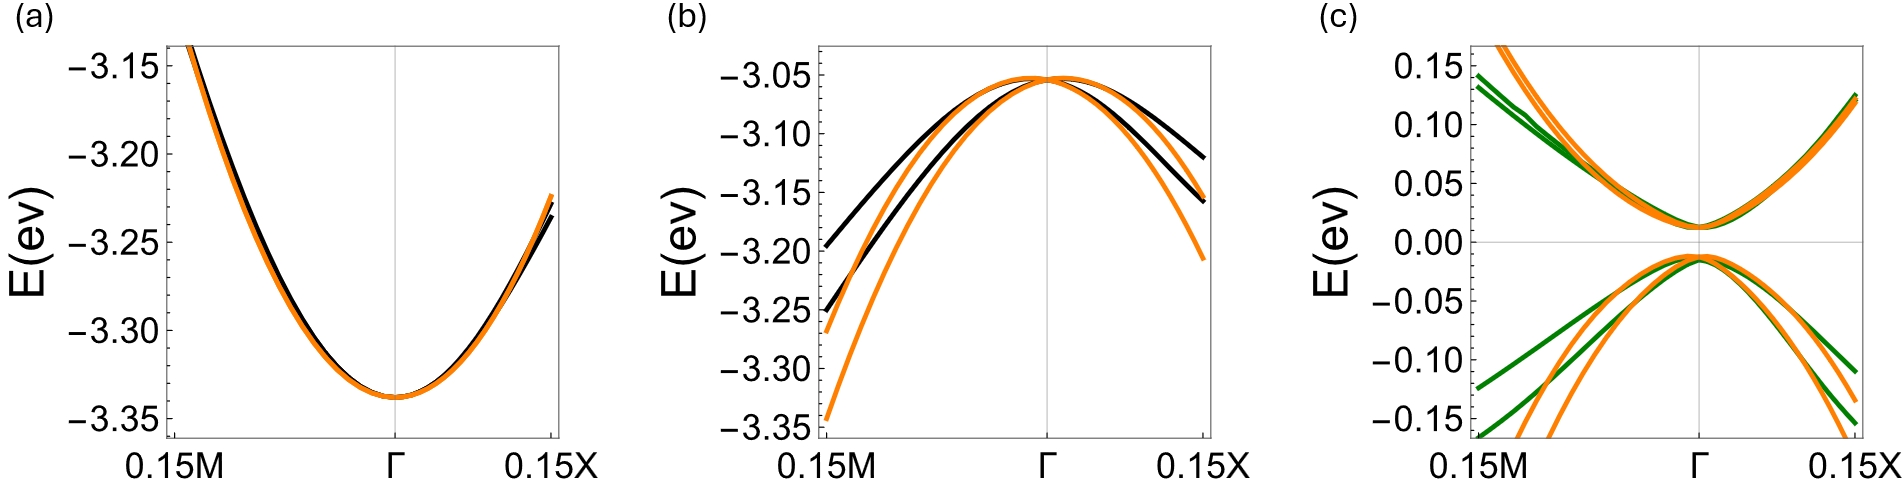
\includegraphics[width=1\textwidth]{images/P-4m2fit.png}
\caption{\justifying 
(a) Band dispersion of the PbS$_2$ conduction bands in the single layer. 
(b) Band dispersion of the TiTe$_2$ valence bands in the single layer. 
(c) Band dispersion of the PbS$_2$/TiTe$_2$ heterostructure. 
In all panels, the DFT bands are shown in black/green, while the orange curves are obtained from the corresponding effective models. 
 \label{fig:P-4m2fit}}
\end{figure}

\begin{table}[h]
\centering
\renewcommand{\arraystretch}{1.2}
\begin{subtable}{1\textwidth}
\begin{tabular}{|c|c|c|c|c|c|c|c|}
\hline
$D_{2d}$ & $\Gamma_1$ & $\Gamma_2$ & $\Gamma_3$ & $\Gamma_4$ & $\Gamma_5$ & $\bar{\Gamma}_6$ & $\bar{\Gamma}_7$ \\
\hline
$E$ & 1 & 1 & 1 & 1 & 2 & 2 & 2 \\
$C_2$ & 1 & 1 & 1 & 1 & -2 & 0 & 0 \\
$2S_4$ & 1 & -1 & 1 & -1 & 0 & $-\sqrt{2}$ & $\sqrt{2}$ \\
$2M_y$ & 1 & 1 & -1 & -1 & 0 & 0 & 0 \\
$C'_2$ & 1 & -1 & -1 & 1 & 0 & 0 & 0 \\
\hline
\end{tabular} 
\caption{}
\end{subtable}
\begin{subtable}{1\textwidth}
\begin{tabular}{|c|c|c|c|c|c|}
\hline
$C_{2v}$ & $\Gamma_1$ & $\Gamma_2$ & $\Gamma_3$ & $\Gamma_4$ & $\bar{\Gamma}_5$ \\
\hline
$C_1$ & $1$ & $1$ & $1$ & $1$ & $2$ \\
$C_2$ & $1$ & $1$ & $-1$ & $-1$ & $0$ \\
$M_y$ & $1$ & $-1$ & $-1$ & $1$ & $0$ \\
$M_x$ & $1$ & $-1$ & $1$ & $-1$ & $0$ \\
\hline
\end{tabular}
\caption{}
\end{subtable}
\caption { \justifying Character tables for the point groups $D_{2d}$ and $C_{2v}$ in (a) and (b), respectively. The irreps with a bar denote double (spinful) representations, while those without a bar correspond to single (spinless) representations.}
\label{Tab:charter table D2d c2v}
\end{table}
\bibliographystyle{apsrev4-2}
\bibliography{references.bib}
\end{document}